\section{ProG：统一的图提示学习工具库}\label{sec:prog}
完善图提示学习生态的关键组成之一，是构建一个高质量、可复用的工程工具。尽管目前已经存在大量面向通用图学习的开源工具，但在“图提示（graph prompt）”这一特定方向上，仍缺乏专门支持提示构建、调优与评测的通用库。为弥补这一空白，我们推出开源统一工具库 \texttt{ProG}（Prompt Graph），其设计目标是面向图提示学习的关键需求，为研究者与工程实践者提供一套灵活、系统、可扩展的实现与评测框架，从而推动图提示方法在更多图任务与真实场景中的落地。

\texttt{ProG} 是一个基于 PyTorch 的工具库，旨在支持对预训练 GNN 的单任务或多任务提示（prompting）。其整体架构如图~\ref{fig:prog} 所示。\texttt{ProG} 集成了图提示评测中常用的多个数据集，包括 Cora、CiteSeer、Reddit、
% ~\cite{hamilton2017inductive},
Amazon
% ~\cite{shchur2019pitfalls},
以及 Pubmed 等。
% ~\cite{kipf2017semisupervised}.
同时，工具库提供了图提示相关任务中常用的评估指标，如 Accuracy、F1 Score 与 AUC 等。值得强调的是，\texttt{ProG} 已集成多种代表性方法，包括 All in One~\cite{sun2023all}、GraphPrompt~\cite{liu2023graphprompt}、GPPT~\cite{sun2022gppt}、GPF~\cite{fang2022prompt} 与 GPF-Plus~\cite{fang2023universal}，并将持续纳入更多图提示模型与基准任务。总体而言，\texttt{ProG} 具有以下关键特性：

\begin{itemize}
    \item \textbf{快速上手。} 所有模型在一致的运行环境下实现，并配备详细示例（demos），便于新用户迅速启动与复现实验。
    \item \textbf{高度模块化。} \texttt{ProG} 采用模块化架构，使你能够按需替换组件并灵活搭建自定义模型与训练流程。
    \item \textbf{易于扩展。} \texttt{ProG} 支持无缝扩展，以便纳入更多方法与更广泛的下游任务，适应不断演进的研究需求。
    \item \textbf{标准化评测。} \texttt{ProG} 提供统一的评测流程与指标口径，促进不同模型之间更公平、可复现的性能对比。
\end{itemize}

\begin{figure}[!t]
    \centering
    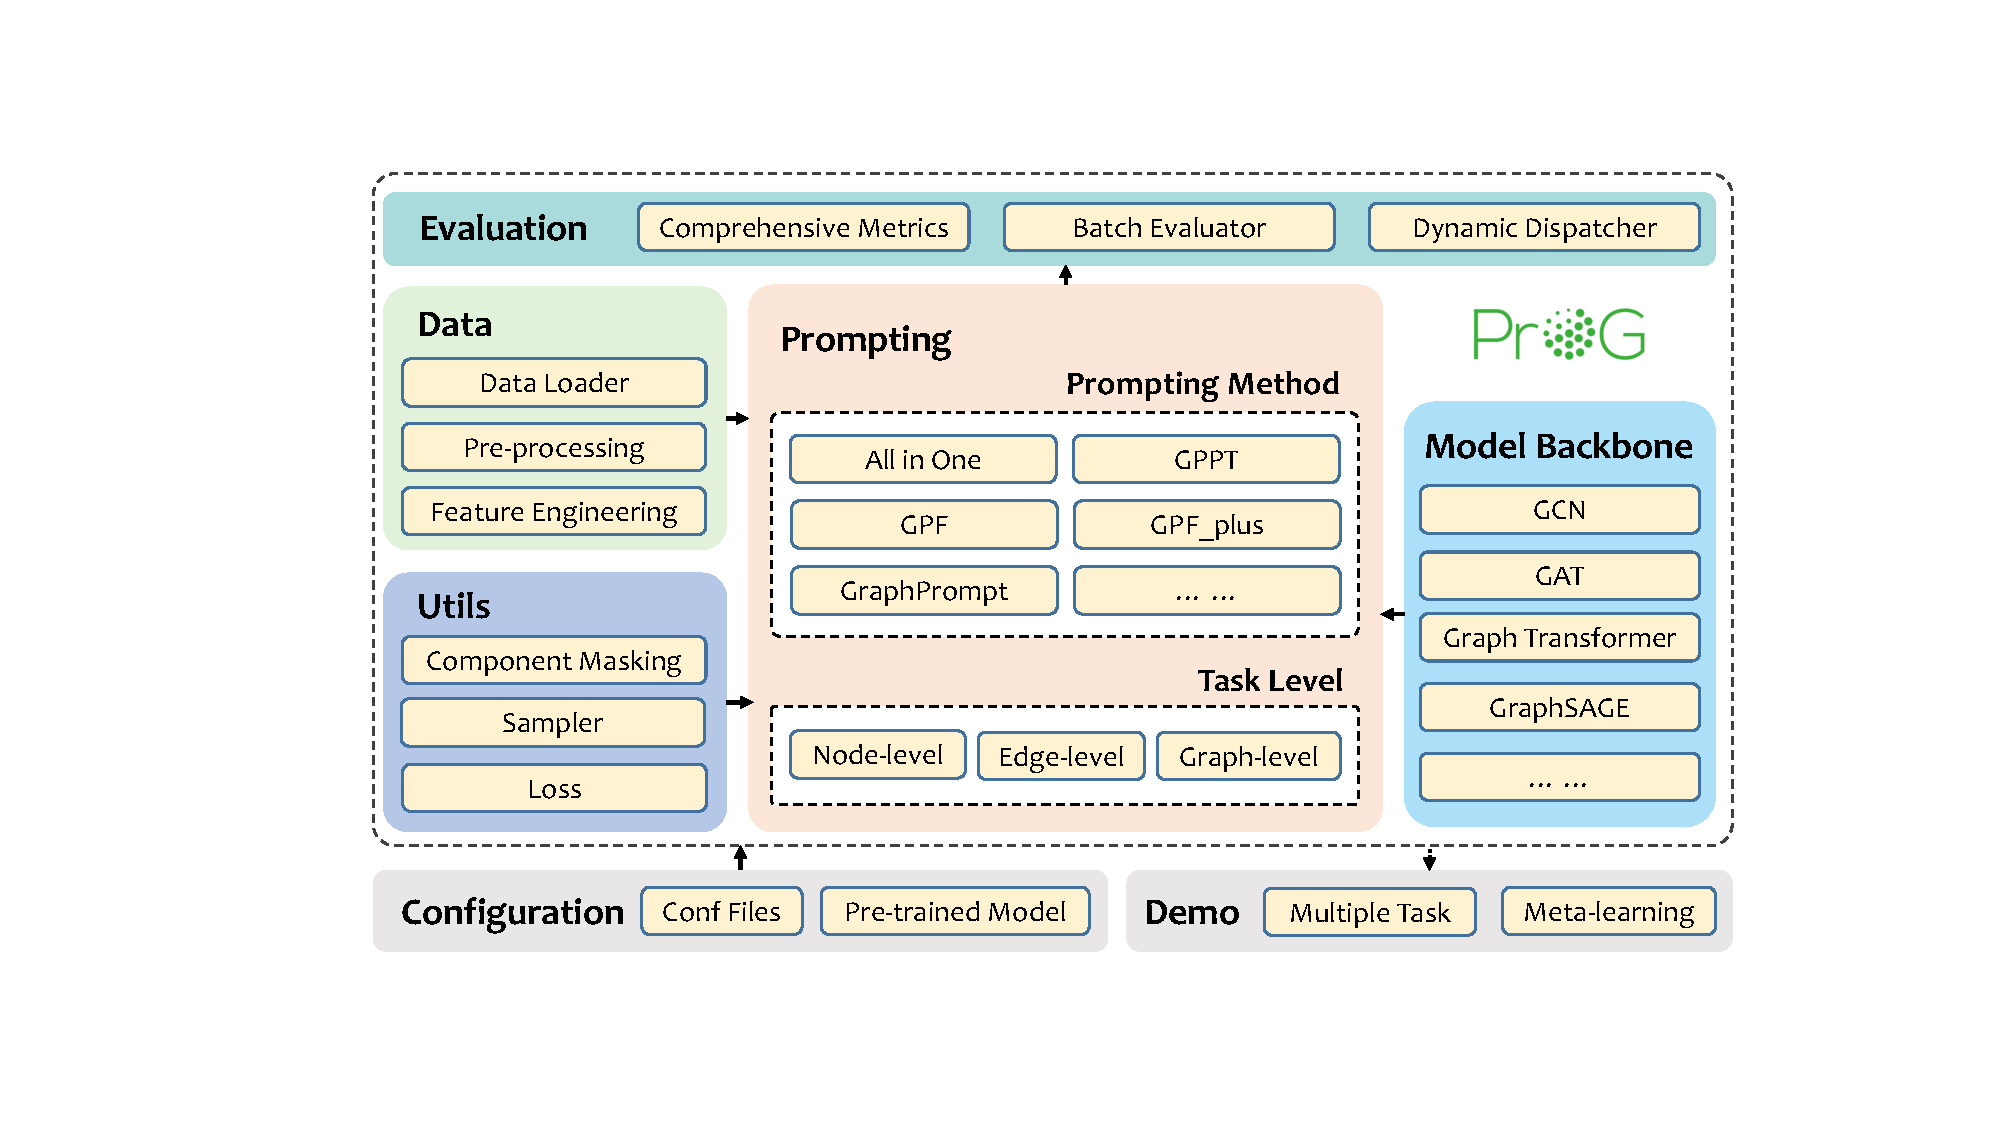
\includegraphics[width=0.5\textwidth]{pic/ProG_pipeline.pdf}
    \caption{ProG 的整体架构。}
    \label{fig:prog}
\end{figure}

如需获取更多信息与访问工具库，请访问我们的项目主页\footnote{\url{https://github.com/sheldonresearch/ProG}}。
此外，我们还维护了一个 GitHub 仓库\footnote{\url{https://github.com/WxxShirley/Awesome-Graph-Prompt}}。
该仓库作为图提示学习最新进展的集中资源库，持续收录并更新相关论文、基准数据集与可用代码实现，从而为该方向的持续研究提供便捷入口与协作平台。
